\documentclass[conference]{IEEEtran}
\IEEEoverridecommandlockouts
% The preceding line is only needed to identify funding in the first footnote. If that is unneeded, please comment it out.
\usepackage{cite}
\usepackage{amsmath,amssymb,amsfonts}
\usepackage[options ]{algorithm2e}
\usepackage{multirow}
\usepackage{listings}
\usepackage{graphicx}
\usepackage{textcomp}
\usepackage{xcolor}
\usepackage{color, colortbl}
\pagenumbering{roman}
\definecolor{Gray}{gray}{0.9}
\def\BibTeX{{\rm B\kern-.05em{\sc i\kern-.025em b}\kern-.08em
    T\kern-.1667em\lower.7ex\hbox{E}\kern-.125emX}}
\begin{document}

\title{Performance of Parallel Matrix Multiplication Algorithms on Blue Gene Q Supercomputer}

\author{
    \IEEEauthorblockN{Jinghua Feng}
    \IEEEauthorblockA{\textit{Department of Computer Science} \\
    \textit{Rensselaer Polytechnic Institute}\\
    Tory NY, US \\
    fengj3@rpi.edu}
\and
    \IEEEauthorblockN{Miao Qi}
    \IEEEauthorblockA{\textit{Department of Computer Science} \\
    \textit{Rensselaer Polytechnic Institute}\\
    Tory NY, US \\
    qim@rpi.edu}
}

\maketitle
\thispagestyle{plain}
\pagestyle{plain}

\begin{abstract}
Matrix multiplication, as a core scientific computation operation, is used to deal with information flow by converting data into machine-readable codes and then back to data. It can be applied in various domains to solve real-life problems such as weather pattern analysis \cite{b1}. However, the data matrices existing in real life usually have large size. The matrix multiplication requires $O(n^3)$ operations, where $n$ is the dimension of a matrix. Therefore, it is time consuming and memory inefficient to execute a sequential algorithm on large matrices. However, the emergence of supercomputers and parallel computing architectures allows previous non-executable or inefficient computations to be done in a reasonable period of time. It leads to the development of parallel algorithms with the goal to minimize the compute execution time through overlapping the computations among processors and to simultaneously increase the overall efficiency by optimizing the data communication pattern between various processors. We have studied two parallel algorithms - the well-known Cannon's algorithm based on the checkerboard data decomposition and the strip algorithm based on the block-striped data decomposition - to solve the matrix multiplication problem with large size matrices. Cannon's algorithm is more memory-efficient while the strip algorithm has less overheads. In our implementation of these two parallel matrix multiplication algorithms in C, we applied Message Passing Interface (MPI), POSIX Threads (Pthreads), and MPI parallel I/O. And we studied the performance of these algorithms by running them on the Blue Gene/Q system using up to 8192 processors. 
\end{abstract}

\begin{IEEEkeywords}
Parallel Computing, Matrix Multiplication, Strong Scaling, Parallel Algorithms
\end{IEEEkeywords}

\section{Introduction}\label{introduction}
Matrix multiplication is one of the most fundamental and critical linear algebra operations used as a building block for scientific computations in various fields such as digital image processing, graph theory\cite{b2}, aerospace engineering, and ocean studies\cite{b3}.  Matrix multiplication is used to solve the following problem: Given two matrices $A$ with size $m \times r$ and $B$ with size $r \times n$, the matrix multiplication algorithm will return a new product matrix $C$ with size $m \times n$. Mathematically, it is $C = A \times B$ and for each element in $C$ we have $c_{ij} = \sum_{k =1}^{r} a_{ik} \times b_{kj}$. Due to the data decomposition scheme for matrices, many widely used algorithms such as Cannon's algorithm \cite{b4} are especially suitable for square matrices with size $n \times n$. Additionally, the input matrices are usually assumed to be equally divisible by the total number of processors in most parallel algorithm designs.

The Blue Gene/Q (BG/Q) system has 5 racks with up to 5120 available nodes \cite{b5}. Each node contains an IBM A2 processor which has 16 cores and runs at 1.6 GHz. It also applies 16 GB of Double Data Rate 3 (DD3) memory. BG/Q is characterized by its low latency and high bandwidth interprocessor connections and memory system to achieve superior performance.  The architecture of BG/Q allows an execution mode of a combination of MPI and threads with faster thread context switching. Its ultra-scalability and extensive applicability can help researchers from various fields to make scientific breakthroughs and advances\cite{b5}. 

The overall performance of the same parallel algorithm may be different based on the architecture of the system that the algorithm is run on. For example, in a shared memory system, since the stored data can be accessed by all processors, synchronization is required to ensure the sequential consistency. On the other hand, in a distributed memory system, since each processor has its own local memory accessible by itself only, information are needed to be exchanged among processors through tools such as MPI to send and receive data from different processors\cite{b2}. So, parallel algorithms with MPI implementation are usually preferred by distributed memory systems. Therefore, to improve the performance of an algorithm on a supercomputer, we need to consider the system's architecture before the implementation.

The rest of the report is organized as follows. In Section \ref{related_works}, we summarize some critical points to improve the efficiency of parallel matrix multiplication algorithms and discuss various existing algorithms based on their purposes.  Section \ref{implementation} presents our implementations for Cannon's algorithm and the proposed strip algorithm using MPI, Pthreads, and I/O operations. Section \ref{results} describes our experimental results from BG/Q and analyzes the performance of two algorithms from various aspects. Conclusions of the project are given in Section \ref{conclusions}. Finally, we talk about the ideas that were not achieved in the current project and some potential future improvements of the algorithms in Section \ref{future_work}. 



\section{Related Works}\label{related_works}
The complexity of the standard sequential matrix multiplication algorithm is $O(n^3)$ since it requires three for loops to iterate each element of the input matrices $A$ and $B$ and compute the result matrix $C$. This sequential algorithm is easily implemented but does not work efficiently when the input data size increases. When the dimension of matrix exceeds some limits, the sequential algorithm fails to return the correct solution as desired. Therefore, various parallel algorithms are developed and implemented to fix the bottleneck of matrix sizes. 

In general, several important aspects should be considered to improve the parallel matrix multiplication algorithm: (1) the layout of submatrices as input for processors; (2) the total number of exchanged messages among processors; (3) the size of message for communication; (4) the data dependency for calculation; (5) the communication pattern between processors for the system; (6) the memory usage; (7) the local computation task for each processor.

Parallel matrix multiplication was first investigated in 1969 \cite{b3}. Some traditional algorithms are described as follows. The systolic algorithm is developed based on systolic synthesis method and uses 1D, 2D, and even higher dimensions of systolic arrays\cite{b6,b7,b8}; the Strassen's matrix multiplication uses the divide-and-conquer method to recursively solve the multiplication on submatrices \cite{b9}; Cannon's  algorithm is a  memory-efficient distributed algorithm applied on square 2D grids and uses cyclic shift operations for data communication \cite{b4}; Fox's algorithm is constructed based on the checkboard scheme for matrix decomposition and performs both cyclic shift and blocks broadcasting operations\cite{b10}; the DNS (Dekel, Nassimi, Sahni) algorithm \cite{b11} is characterized by its 3D matrix partitioning scheme for dense matrix multiplication; Parallel Universal Matrix Multiplication (PUMMA) is extended from the Fox's algorithm to non-square matrices based on the block scattered data distribution and is designed for distributed memory concurrent computers \cite{b12, b13} ; BiMMeR's algorithm is another extension from the Fox's algorithm to non-square matrices but for a different data layout called virtual 2-D torus wrap \cite{b14}; Scalable Universal Matrix Multiplication (SUMMA) is a highly efficient and scalable algorithm that requires less work space\cite{b15}; and the generalized sparse matrix-matrix multiplication (SpGEMM) works efficiently for sparse matrices using a two-dimensional block data distribution \cite{b16}.

According to the heavy demand of matrix multiplication in scientific studies, several advanced algorithms are developed. Distribution Independent Matrix Multiplication (DIMMA) is very similar to SUMMA and is designed for distributed-memory concurrent computers based on block cyclic data distribution \cite{b17}. It implements two new ideas: first, its modified pipelined communication scheme maximizes the overlap of computations and improves the efficiency for data communication; second, its LCM block concept allows for optimal performance of the sequential BLAS routine on both small and large block sizes\cite{b17}. The Sub Tasks Matrix Multiplication Algorithm (STMMA) \cite{b3} can overcome the following four drawbacks simultaneously: first, it can be applied to non-square matrices; second, it finds the optimal block size; third,it offers optimal number and size for the data chunks transferred among processors; fourth, it tries to minimize the data dependency. Shared and Remote-memory based Universal Matrix Multiplication Algorithm (SRUMMA) is designed for dense matrices running on systems with shared memory and clusters\cite{b18}. Instead of using the traditional message passing approach, SRUMMA explicitly exploits the remote memory access (RMA) and shared memory for data communication.

Even though all the above algorithms are designed for matrix multiplication, there are some differences for their usage. In general, most matrix multiplication algorithms can be classified based on four aspects. First, as mentioned in Section \ref{introduction}, algorithms are designed differently for shared memory system and distributed memory systems to improve the data communication based on the parallel computer paradigms \cite{b2}. For instance, DIMMA is for distributed memory systems while SRUMMA is for shared memory system. Second, in real world, data matrices may be dense or sparse. So different algorithm designs are necessary for sparse-sparse, dense-dense, and dense-sparse matrix product problems to reduce the computational complexity and achieve faster calculations \cite{b19,b20}.  Third, for a large matrix, the data can be decomposed to several strips of continuous rows or columns or to be partitioned into a set of blocks like the checkboard \cite{b21}. Most of the well-known parallel matrix multiplication algorithms depend on the checkboard data decomposition. Fourth, some algorithms requires the input matrices to be square while others allow for the rectangular matrix multiplication \cite{b22}. These aspects work together to generate various algorithms. For instance, the algorithm proposed by Coppersmith \cite{b22} can be applied to rectangular matrices while Cannon’s and Fox’s algorithms are usually applied to square matrices. 



\section{Implementation of Parallel Algorithms}\label{implementation}

\subsection{Cannon's Algorithm}
Cannon's algorithm divides matrices $A$ and $B$ into $p$ square submatrices with size of $\frac{n}{\sqrt{p} } \times \frac{n}{\sqrt{p}}$. $A^{ij}$ and $B^{ij}$ are used to denote sub-blocks residing with processor $(i,j)$. As shown in Figure \ref{mat_init}, the submatrices of $A$ and $B$ is aligned by sending the block $A^{ij}$ to processor $(i,(j+i)\%\sqrt{p})$ and sending the block $B^{ij}$ to processor $((i+j), j)\%\sqrt{p})$, respectively. After multiplying the copied two sub-blocks to obtain initial $C$, A sub-blocks and B sub-blocks are rolled one sub-block left and one sub-block upward respectively, as shown in Figure \ref{mat_shift}, and then multiplied together to add to $C$. Repeating $\sqrt{p}$ steps of rolling, multiplying, and summation, the final $C$ is obtained.

The running time of Cannon's algorithm consists of parallel execution time $T_p$, data communication costs $t_s$ and $t_w$, where $t_s$ and $t_w$ are the message startup time and communication time per word ($\frac{y}{B}$, $y$ is number of bytes per word, $B$ is bandwidth with unit of bytes/second), respectively. The initial alignment takes much less time than the time spent in the multiplication phase when the number of  processors is large. That's because the initial alignment is one-iteration communication compared with $\sqrt{p}$ rolling in the multiplication phase. As each block movement in the multiplication phase takes $t_s+t_w\frac{n^2}{p}$ time, the total running time is
\begin{equation}
    T_p = \frac{n^3}{p} + 2t_s\sqrt{p} + 2t_w\frac{n^2}{\sqrt{p}})
\label{eq_cannon_runtime}
\end{equation}

The main steps to implement Cannon's algorithm are shown in Algorithm \ref{alg:cannon}.

% -------- Cannon Algorithm ---------------- 
\begin{figure}[!h]
    \centering
    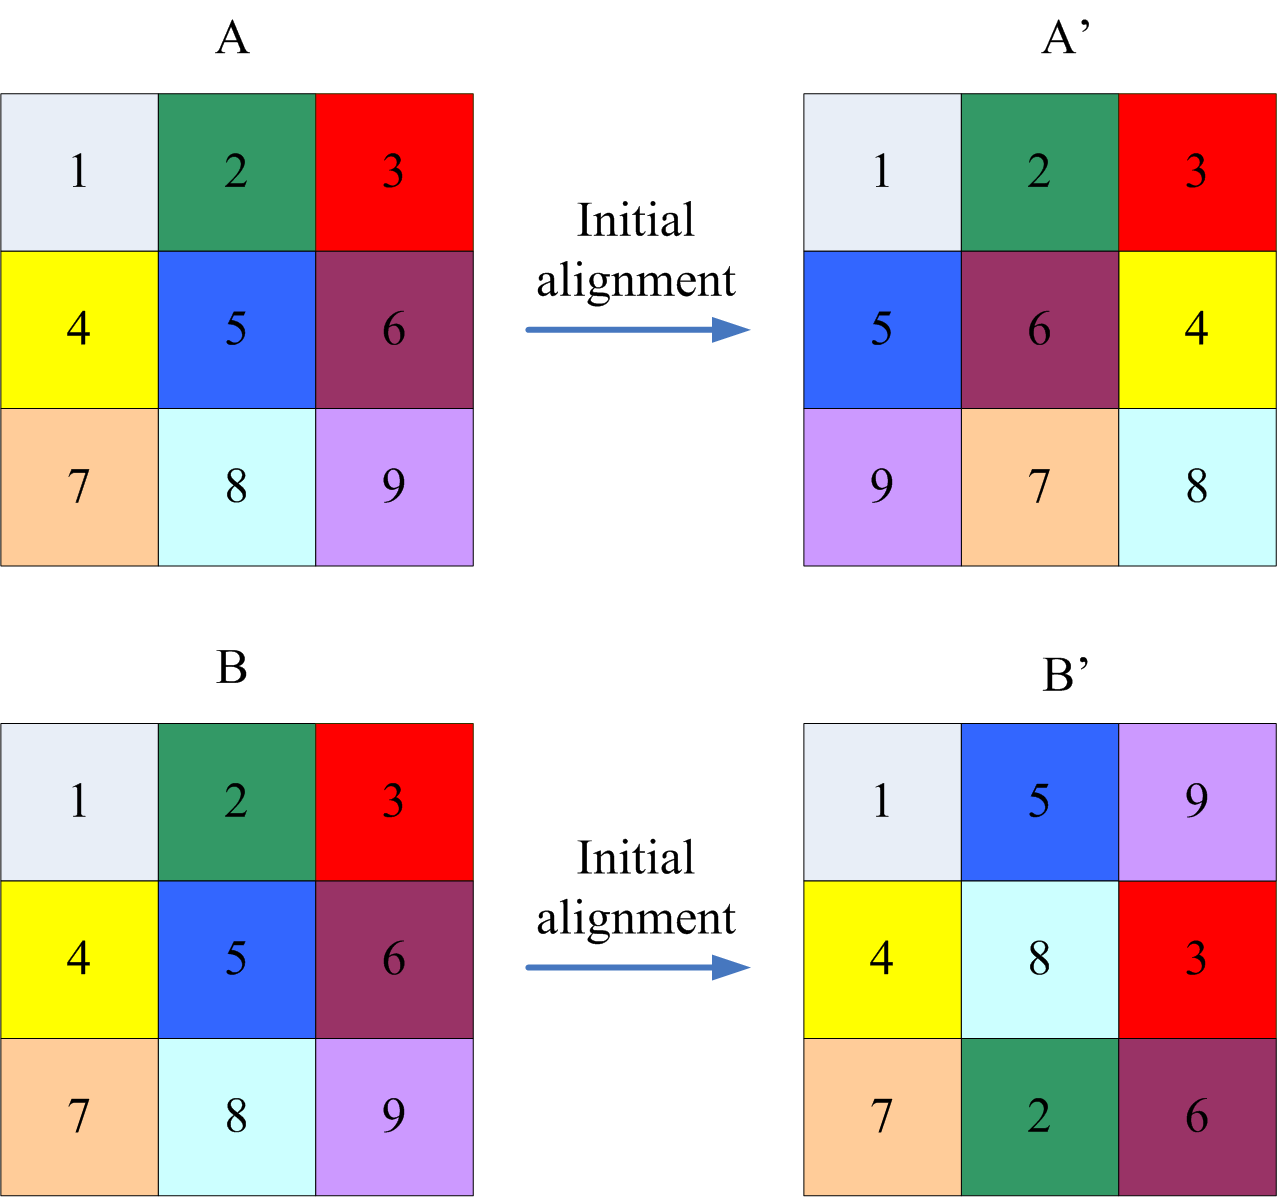
\includegraphics[scale=0.4]{Figures/cannon/init_align.png}
    \caption{ Initial alignment of matrices A and B( The sub-blocks at row $i$ of $A$ are rolled $i$ steps leftwards; The sub-blocks at column $j$ of $B$ are rolled $j$ steps upwards}
    \label{mat_init}
\end{figure}
\begin{figure}[!h]
    \centering
    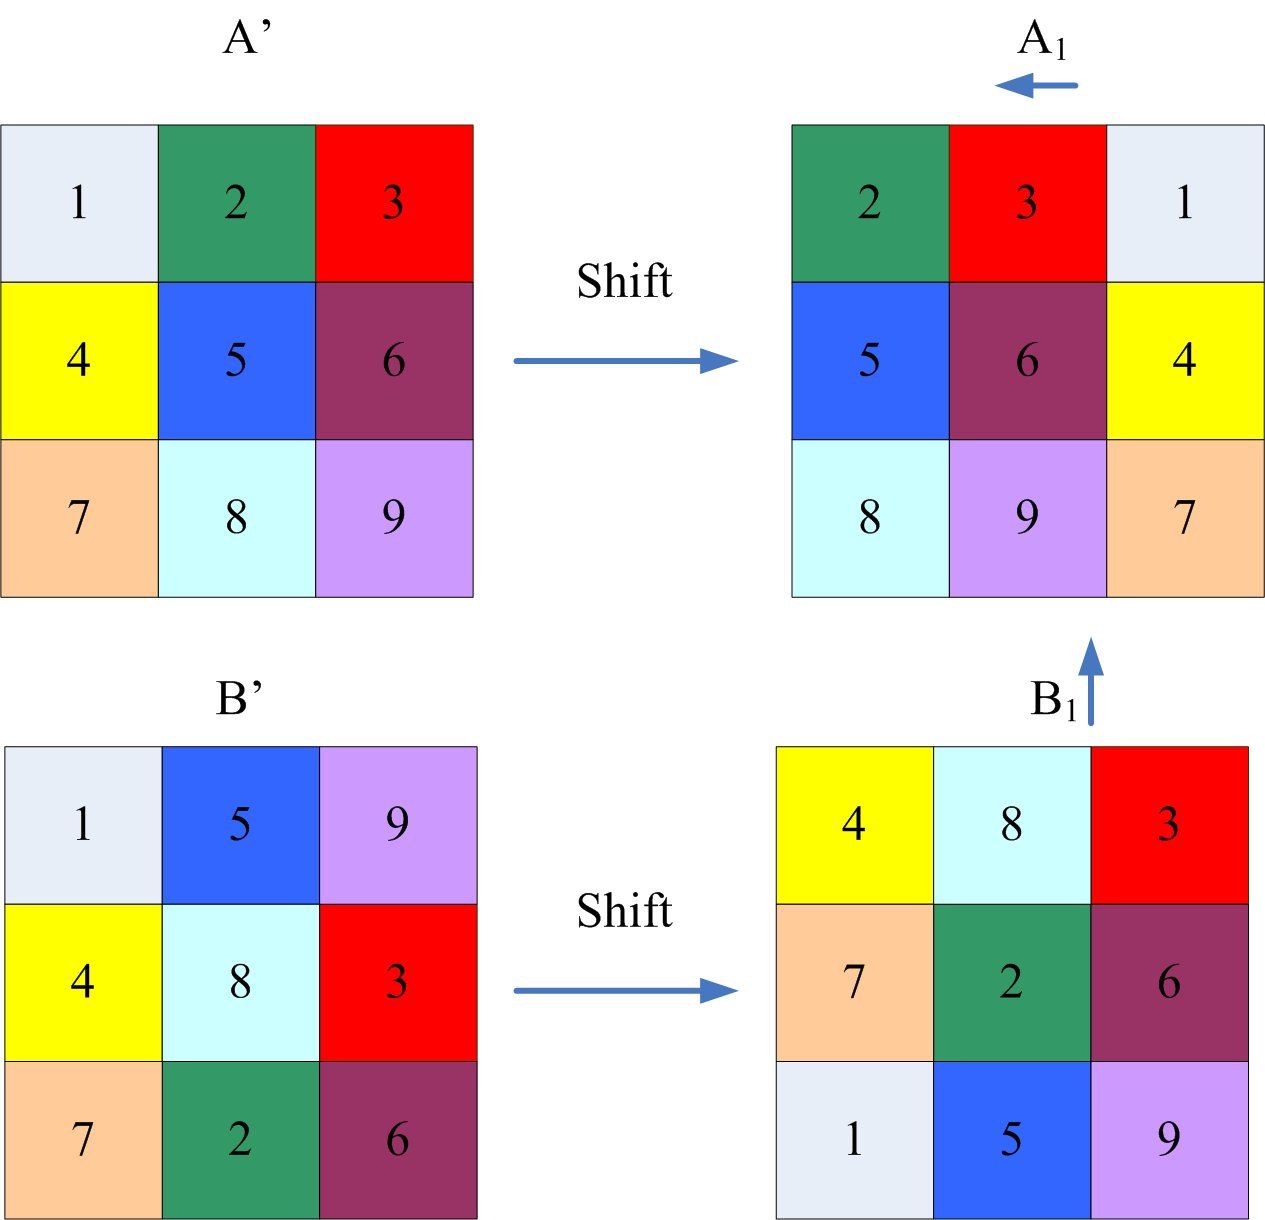
\includegraphics[scale=0.4]{Figures/cannon/rolling.png}
    \caption{ Rolling one sub-block for matrices $A'$ and $B'$ at first iteration during multiplication phase ($A'$ moves one sub-block leftwards, $B'$ moves one sub-block upwards)}
    \label{mat_shift}
\end{figure}

\begin{algorithm}
\SetAlgoLined
\KwIn{$A$: a $n \times n $ matrix ; $B$: a $n \times n $ matrix }
\KwOut{$C$: a $n \times n $ matrix }
 \Begin
  {Step 1: Initialize MPI\;
   Step 2: Compute number of sub-blocks in each row and number of rows in each square sub-block\;
   Step 3: Dynamically allocate and initialize $A\_block$, $B\_block$, and $C\_block$ as 1D arrays\;
   Step 4: Create Cartesian topology, initialize ranks and coordinates in new Cartesian topology\;
   Step 5: Align matrices $A$ and $B$: compute shift coordinates by MPI\_Cart\_shift(), use MPI\_Sendrecv\_replace() to roll sub-blocks\; 
   Step 6: Compute rank number for left, right, top, and bottom shift\;
   Step 7: Roll sub-blocks and perform sub-block matrix multiplication\\
        \For{MPI rank $i = 0 \cdots  num\_ranks$}{ 
        Step 6.1: Roll sub-blocks $A\_block$ and $B\_block$ to targeted positions by MPI\_Isend() and MPI\_Irecv()\;
        Step 6.2: Compute serially matrix multiplication of sub-block $A\_block$ and $B\_block$, sum the results to $C\_block$\;
        Step 6.3: Apply MPI\_Wait() for MPI\_Isend/Recv()
         }
    Step 8: Write $C\_block$ to a common file concurrently\;
        \For{MPI rank $i = 0 \cdots  num\_ranks$}{ 
        Step 6.1: Compute initial offset based on rank number\;
        Step 6.2: 
            \For{Row $j = 0 \cdots rows\_block$}{ 
                Write row $j$ of $C\_block$ to the right position of file by collective MPI\_File\_write\_at\_all()\;
                Update offset\;
            }
         }
    Step 9: If rank 0 / thread 0, end to record execution time with GetTimeBase()\;
    Step 10: Deallocate memory and finalize MPI.
  }
 \End
 \caption{Cannon's algorithm}
 \label{alg:cannon}
\end{algorithm}



\subsection{Strip Algorithm}

The strip algorithm designed based on the block-striped data decomposition is developed from the sequential algorithm. Since the sequential algorithm takes a long time to calculate the result for matrices with large size, it is reasonable to assign subtasks to multiple processors for parallel computation. However, to design subtasks that can improve the performance of our algorithm, we should consider two factors: first, for the aspect of overheads, the total number of subtasks should not be extremely large (e.g. each row of two input matrices are assigned to a different processor) to cause enormous overheads for data communication; second, for the aspect of parallelism, the total number of subtasks should not be very small to avoid taking advantage of parallel computation. 

This parallel algorithm requires less communication between processors compared to other parallel approaches, and it can be easily implemented through a combination of MPI and Pthreads. However, it is not very memory efficient and may cause excessive memory usage to affect the final result calculation. So, this algorithm is not implemented as a parallel algorithm in most of the existing research related to matrix multiplication. But we plan to achieve it in our research by applying shared memory processes such as Pthreads. If the number of threads per MPI rank is carefully designed based on the system architecture, this algorithm should be competitive to other parallel algorithms in total running time since it has very few overheads. Additionally, it can be embedded in other parallel algorithms such as the Cannon's algorithm which is difficult to add in Pthreads to optimize the efficiency and benefit from the light weights of Pthreads.

The Algorithm \ref{alg:simple} describes the main steps of our strip algorithm. After setting up the MPI, we assigned each rank with some rows of the input matrix $A$. If threads are needed, we assign the computational work to each thread equally and collect results from them later. MPI ranks are regarded as threads and will perform a subtask as other pthreads to maximize the parallelism of computation. After all ranks finish their work, we put the local results into a global result matrix.

\begin{algorithm}[H]
\SetAlgoLined
\KwIn{$A$: a $n \times n $ matrix ; $B$: a $n \times n $ matrix }
\KwOut{$C$: a $n \times n $ matrix }
 \Begin
  {Step 1: Setup MPI\;
   Step 2: Compute the number of rows of matrix A assigned to each rank\;
   Step 3: Dynamically allocate and initialize $A\_local$, $B$, and $C\_local$ as 1D arrays\;
   Step 4: If rank 0 / thread 0, start to record execution time with GetTimeBase()\;
   Step 5: Setup Pthreads\; 
   Step 6:\\
        \For{each MPI rank and thread $i = 0 \cdots  num\_threads$}{ 
        Step 6.1: Compute the number of rows of matrix A assigned to each thread\;
        Step 6.2: Calculate the start index and end index for the thread to process\;
        Step 6.3: Apply the function \textbf{StripMatrix} to the $A[j \cdots l]$ and $B$, where $j$ is the first element and $l$ is the last element assigned to the MPI/thread
         }
    Step 7: Clean the threads\;
    Step 8: Use MPI\_Gather to collect results from each MPI rank to $C$\;
    Step 9: If rank 0 / thread 0, end to record execution time with GetTimeBase()\;
    Step 10: Free dynamically allocated memory.
  }
 \End
 \caption{The strip algorithm based on block-striped data decomposition}
 \label{alg:simple}
\end{algorithm}

 
The Algorithm \ref{alg:stripmatrix} explains the method used to do the local calculation of each subtask. In general, it is a sequential algorithm for matrix multiplication performed on a subtask.\\

\begin{algorithm}[H]
\SetAlgoLined
\KwIn{$A'$: a $k \times n $ matrix ; $B$: a $n \times n $ matrix }
\KwOut{$C'$: a $k \times n $ matrix }
 \Begin
  {Step 1: Apply the standard sequential Matrix Multiplication to $A'$ and $B'$ to calculate $C'$
  }
 \End
 \caption{ The function \textbf{StripMatrix}}
 \label{alg:stripmatrix}
\end{algorithm}

The Listing 1 shows the implementation of the above \textbf{StripMatrix} algorithm with a helper function called \textbf{UnsquareMultiplication}. The function \textbf{UnsquareMultiplication} can calculate the product of two matrices with different sizes (i.e. the two input matrices are not necessary to be $n \times n$ but need to satisfy the dimension rules for matrix multiplication). 
\lstset{ basicstyle=\footnotesize,breakatwhitespace=false,breaklines=true, tabsize = 2}
\lstinputlisting[language=c,caption={C code for the StripMatrix function based on the sequential matrix multiplication algorithm},label=DescriptiveLabel]{StripMatrix.c}


\section{Experimental Results and Discussion}\label{results}
We write a C function to automatically generate matrices as our input for testing. Currently, the program can initialize the matrices (1) based on their global indices, (2) to all ones, (3) to all zeros, and (4) to some random numbers with user input constraints. 

To study the overall performance of the two algorithms described in the previous section on the BG/Q system, we design the experiments as the following: 
\begin{itemize}
    \item Cannon's Algorithm: as Cannon's algorithm requires the number of MPI ranks to be square of an integer, we execute the Cannon's program by applying 1, 4, 16, 64 compute nodes (without using 32 and 128 nodes) with 64 tasks per node. To see the influence of matrix size on the execution, we run the algorithm with 4 different matrix size: $1024\times1024$, $2048\times2048$, $4096\times4096$, $8192\times8192$. The data types for data matrices can be easily set up if necessary. To save memory and I/O time, we only illustrate the experimental results for integer matrices below.
    \item Strip Algorithm: we run this algorithm with 4, 8, 16, 64, and 128 compute nodes. For each different number of compute nodes, we use 5 different threads per MPI rank ratio: 4 threads per rank (i.e. 16 MPI ranks and 48 Pthreads per compute node), 8 threads per rank (i.e. 8 MPI ranks and 56 Pthreads per compute node), 16 threads per rank (i.e. 4 MPI ranks and 60 Pthreads per compute node), 32 threads per rank (i.e. 2 MPI ranks and 62 Pthreads per compute node), and 64 threads per rank (i.e. 1 MPI ranks and 63 Pthreads per compute node). So, we have a total of 25 experiments performed on BG/Q. Our input matrix have a size of 8192 * 8192 to allow the algorithm to be successfully executed using up to 128 compute nodes. 
\end{itemize}

To evaluate the correctness of our implementations for both algorithms, we generate matrices with different sizes and numbers using the combination of the 4 different kinds of initialization setup described above. After applying our algorithms to these matrices, we proved the correctness of the calculation through online calculators and the sequential algorithm for matrices with reasonable sizes. 

\subsection{Cannon's Algorithm}
%-----------------------------------------------------------------
% Execution time and Speedup
%-----------------------------------------------------------------
\subsubsection{Execution time and Speedup ratio}\\
The total execution time of Cannon's algorithm versus number of MPI ranks is displayed in Figure \ref{cannon_exe} and in Table \ref{cannon_tb_exe}. The results show that the execution time decreases with the increasing number of MPI ranks. The execution time typically increases around 8 times as the matrix size doubles, which is consistent with Equation \ref{eq_cannon_runtime}. But for the matrices of small size ($1024\times1024$, $2048 \times 2048$), it does not satisfy Equation \ref{eq_cannon_runtime} at $4096$ MPI ranks. The reason is that the real execution time (time consumed by real matrix multiplication) with large number of MPI ranks (i.e.,$4096$) is very small, which may be comparable to overhead of Cannon's algorithm. By using the execution time of 1 node (64 MPI ranks) to compute the multiplication of $8192\times8192$ matrices as the base, we obtain the speedup ratios in Figure \ref{cannon_spd} and Table \ref{cannon_tb_spd}, which indicates that the speedup increases with increase of MPI ranks. Similarly, the speedup ratio does not have obvious increase when matrix rise from $1024$ to $2048$ at $4096$ MPI ranks. 
% -------- Figure: execution time ----------------
\begin{figure}[!h]
    \centering
    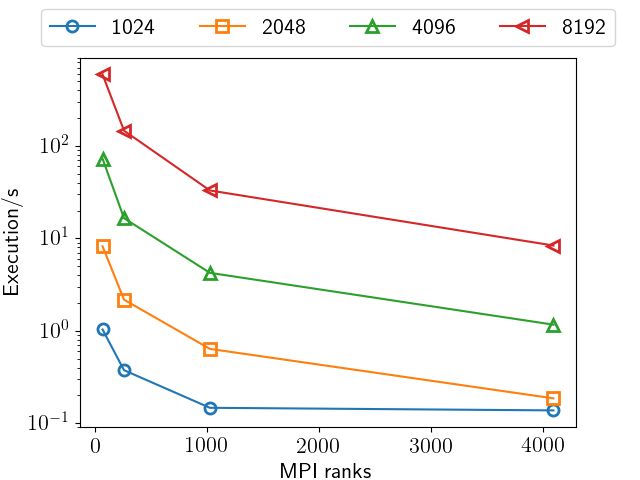
\includegraphics[scale=0.4]{Figures/cannon/execution_vs_ranks.png}
    \caption{ Execution time at different \# of MPI ranks for multiplying matrices with different size (1024$\times$1024, 2048$\times$2048, 4096$\times$4096, 8192$\times$8192)}
    \label{cannon_exe}
\end{figure}
% -------- Table: execution time ----------------
\newcolumntype{g}{>{\columncolor{Gray}}c}
\begin{table}[!ht]
\caption{Execution time for different MPI ranks and matrix sizes} \label{cannon_tb_exe} 
\centering
\begin{tabular}{c|g|g|g|g}
\hline
\rowcolor{white}
& \multicolumn{4}{c}{\# MPI ranks}\\
\hline
\rowcolor{white}
\# Matrix size &64 &256 &1024 &4096 \\
\hline
\rowcolor{white}
1024 & 1.033 &  0.375 &  0.147 &  0.138 \\
2048 & 8.201 &  2.171 &  0.637 &  0.186 \\
\rowcolor{white}
4096 & 72.806 & 16.529 & 4.233 & 1.165 \\
8192 & 593.065 & 146.024 & 32.950 & 8.360 \\
\hline
\end{tabular}
\end{table}

% -------- Figure: Speedup ratio ----------------
\begin{figure}[!h]
    \centering
    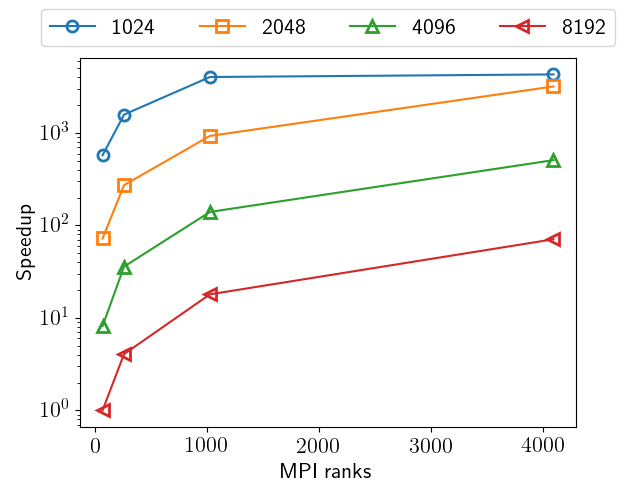
\includegraphics[scale=0.4]{Figures/cannon/speedup.png}
    \caption{ Speedup ratios at different \# of MPI ranks for multiplying matrices with different size (1024$\times$1024, 2048$\times$2048, 4096$\times$4096, 8192$\times$8192)}
    \label{cannon_spd}
\end{figure}
% -------- Table: Speedup ratio ----------------
\newcolumntype{g}{>{\columncolor{Gray}}c}
\begin{table}[!ht]
\caption{Speedup ratios for different MPI ranks and matrix sizes} \label{cannon_tb_spd} 
\centering
\begin{tabular}{c|g|g|g|g}
\hline
\rowcolor{white}
& \multicolumn{4}{c}{\# MPI ranks}\\
\hline
\rowcolor{white}
\# Matrix size &64 &256 &1024 &4096 \\
\hline
\rowcolor{white}
1024 & 574.198 & 1582.153 & 4035.968 & 4306.499 \\

2048 & 72.320 & 273.136 & 930.837 & 3189.929 \\
\rowcolor{white}
4096 & 8.146 & 35.880 & 140.114 & 509.185 \\

8192 & 1.000 & 4.061 & 17.999 & 70.942 \\

\hline
\end{tabular}
\end{table}

%-----------------------------------------------------------------
% Parallel efficiency
%-----------------------------------------------------------------
\subsubsection{Parallel efficiency}
Parallel efficiency is computed via dividing speedup by the number of processors (MPI ranks). The results are illustrated in Figure \ref{cannon_eff} and Table \ref{cannon_tb_eff}. The efficiencies for matrix size of $8192\times8192$, and $4096\times4096$ display strong scalability, i.e., keeping the same with rising MPI ranks. There is a slight decrease of efficiency with increasing ranks for matrix size of $2048\times2048$. For matrix size of $1024\times1024$, it has a dramatic decrease with rising MPI ranks. We have the similar explanation for this observation, that is, the overhead accounts for large portion of the total execution time at large MPI ranks.
% -------- Figure: Efficiency ----------------
\begin{figure}[!h]
    \centering
    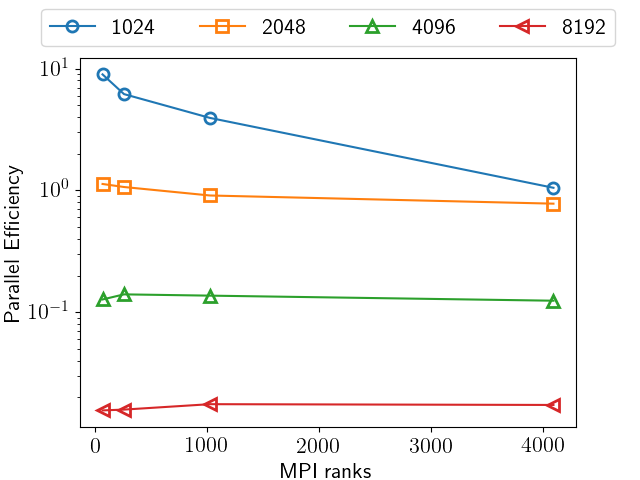
\includegraphics[scale=0.4]{Figures/cannon/efficiency.png}
    \caption{ Parallel efficiencies at different \# of MPI ranks for multiplying matrices with different size (1024$\times$1024, 2048$\times$2048, 4096$\times$4096, 8192$\times$8192)}
    \label{cannon_eff}
\end{figure}
% -------- Table: Efficiency ----------------
\newcolumntype{g}{>{\columncolor{Gray}}c}
\begin{table}[!ht]
\caption{Parallel efficiency for different MPI ranks and matrix sizes} \label{cannon_tb_eff} 
\centering
\begin{tabular}{c|g|g|g|g}
\hline
\rowcolor{white}
& \multicolumn{4}{c}{\# MPI ranks}\\
\hline
\rowcolor{white}
\# Matrix size &64 &256 &1024 &4096 \\
\hline
\rowcolor{white}
1024 & 8.972 & 6.180 & 3.941 & 1.051 \\

2048 & 1.130 & 1.067 & 0.909 & 0.779 \\
\rowcolor{white}
4096 & 0.127 & 0.140 & 0.137 & 0.124 \\

8192 & 0.016 & 0.016 & 0.018 & 0.017 \\
\hline
\end{tabular}
\end{table}

%-----------------------------------------------------------------
% Overhead analysis
%-----------------------------------------------------------------
\subsubsection{Real time vs. Overhead}
Cannon's algorithm mainly consists of three types of overheads:
\begin{itemize}
    \item Communication cost for sub-block rolling at Step 6.1 in Algorithm \ref{alg:cannon}: this type of overhead is generated by communication function calls such as MPI\_Isend(), MPI\_Irecv() and corresponding MPI\_Wait();
    \item Cost for setting up Cartesian topology at Step 4 in Algorithm \ref{alg:cannon}: this includes creation of cart topology by MPI\_Cart\_Create(), initialization of Cartesian ranks by MPI\_Comm\_ranks, and initialization of Cartesian coordinates by MPI\_Cart\_coords();
    \item Cost of initial alignment for matrices $A$ and $B$ at Step 5: containing the time spent on computing shift coordinates by MPI\_Cart\_shift(), and the time taken on rolling sub-blocks by MPI\_Sendrecv\_replace(); 
\end{itemize}
We record the three types of overheads, which are displayed together with total execution time, and real execution time (time spent on block sereial matrix multiplicaton) in Figure \ref{cannon_distb_1024}, \ref{cannon_distb_2048}, \ref{cannon_distb_4096}, and \ref{cannon_distb_8192} for the four different matrix size respectively. The real execution time and the three overheads are also illustrated in Table \ref{cannon_tb_real}, \ref{cannon_tb_settop}, \ref{cannon_tb_align}, and \ref{cannon_tb_comm}, respectively. From these Figures and Tables, we have several observations and corresponding explanations below:
\begin{itemize}
    \item Time spent on setting up Cartesian topology is independent on matrix size. It has a significant increase when number of MPI ranks rises from 64 (1 compute node) to 256 (4 compute nodes).
    \item Time spend on the initial alignment decreases with the rising MPI ranks. This is easy to understand: more MPI ranks generate smaller local sub-blocks for each rank, leading to smaller size of communication data for each MPI rank.
    \item For large matrix size, communication cost for sub-block rolling during matrix multiplication decreases during first three MPI ranks, then has a slight increase from 1024 to 4096 MPI ranks. 
    \item The lines for real execution time and total execution time almost overlap for all MPI ranks at large matrix size, but deviate at larger MPI ranks for small matrix size. This result provides solid proof for the above observation in Figure \ref{cannon_exe} that the execution time does not satisfy Equation \ref{eq_cannon_runtime} at $4096$ MPI ranks when matrix size increases from 1024 to 2048. Apparently, the main overhead for small matrix size comes from setting up MPI Cart topology, which is larger than the real time at MPI rank 1024, 4096 for matrix size 1024, and at MPI rank 4096 for matrix size 2048.
\end{itemize}
% -------- Time distribution ----------------
\begin{figure}[!h]
    \centering
    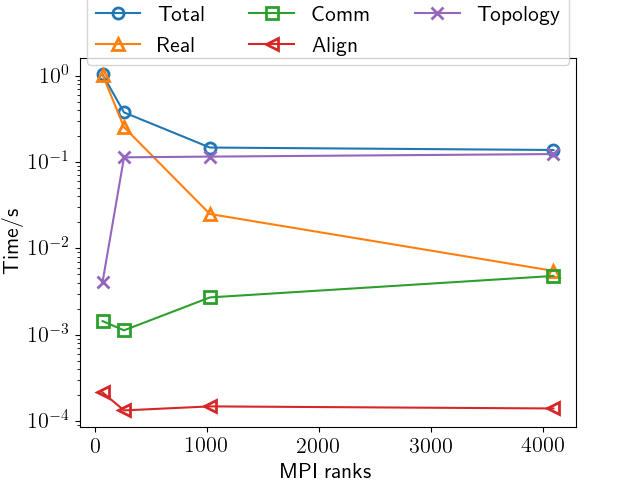
\includegraphics[scale=0.4]{Figures/cannon/time_distribute_1024.png}
    \caption{ Time distribution at different \# of MPI ranks with matrix size 1024$\times$1024}
    \label{cannon_distb_1024}
\end{figure}

\begin{figure}[!h]
    \centering
    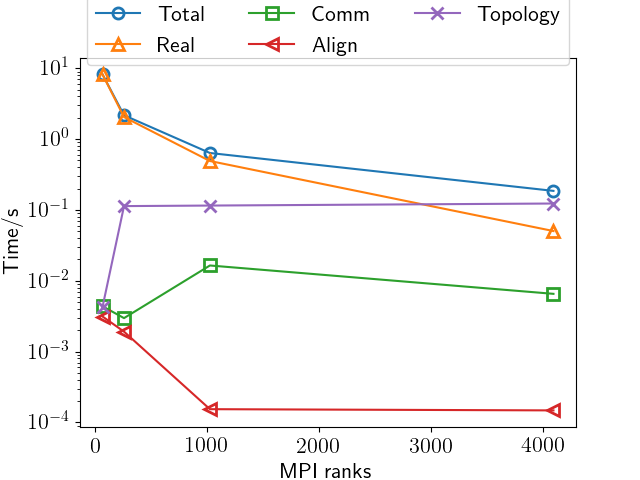
\includegraphics[scale=0.4]{Figures/cannon/time_distribute_2048.png}
    \caption{ Time distribution at different \# of MPI ranks with matrix size 2048$\times$2048}
    \label{cannon_distb_2048}
\end{figure}

\begin{figure}[!h]
    \centering
    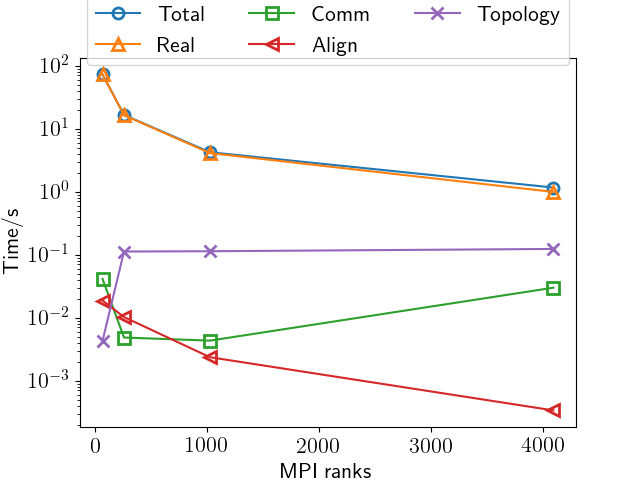
\includegraphics[scale=0.4]{Figures/cannon/time_distribute_4096.png}
    \caption{ Time distribution at different \# of MPI ranks with matrix size 4096$\times$4096}
    \label{cannon_distb_4096}
\end{figure}

\begin{figure}[!h]
    \centering
    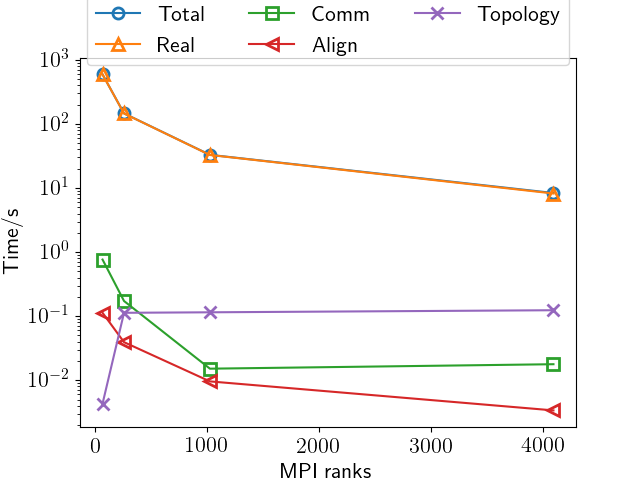
\includegraphics[scale=0.4]{Figures/cannon/time_distribute_8192.png}
    \caption{ Time distribution at different \# of MPI ranks with matrix size 8192$\times$8192}
    \label{cannon_distb_8192}
\end{figure}
% -------- Table: real time ----------------
\newcolumntype{g}{>{\columncolor{Gray}}c}
\begin{table}[!ht]
\caption{Real time for different MPI ranks and matrix sizes} \label{cannon_tb_real} 
\centering
\begin{tabular}{c|g|g|g|g}
\hline
\rowcolor{white}
& \multicolumn{4}{c}{\# MPI ranks}\\
\hline
\rowcolor{white}
\# Matrix size &64 &256 &1024 &4096 \\
\hline
\rowcolor{white}
1024 & 1.023 & 0.253 & 0.025 & 0.005 \\

2048 & 8.181 & 2.049 & 0.491 & 0.050 \\
\rowcolor{white}
4096 & 72.737 & 16.388 & 4.107 & 0.993 \\

8192 & 592.014 & 145.628 & 32.776 & 8.211 \\

\hline
\end{tabular}
\end{table}

% -------- Table: Setup cartesian topology time ----------------
\newcolumntype{g}{>{\columncolor{Gray}}c}
\begin{table}[!ht]
\caption{ Time consumed by setting up Cartesian topology for different MPI ranks and matrix sizes} \label{cannon_tb_settop} 
\centering
\begin{tabular}{c|g|g|g|g}
\hline
\rowcolor{white}
& \multicolumn{4}{c}{\# MPI ranks}\\
\hline
\rowcolor{white}
\# Matrix size &64 &256 &1024 &4096 \\
\hline
\rowcolor{white}
1024 & 0.001 & 0.001 & 0.003 & 0.005 \\

2048 & 0.004 & 0.003 & 0.016 & 0.007 \\
\rowcolor{white}
4096 & 0.041 & 0.005 & 0.004 & 0.030 \\

8192 & 0.764 & 0.173 & 0.015 & 0.018 \\
\hline
\end{tabular}
\end{table}

% -------- Table: Initial alignment time ----------------
\newcolumntype{g}{>{\columncolor{Gray}}c}
\begin{table}[!ht]
\caption{ Time consumed by initial alignment for different MPI ranks and matrix sizes} \label{cannon_tb_align} 
\centering
\begin{tabular}{c|g|g|g|g}
\hline
\rowcolor{white}
& \multicolumn{4}{c}{\# MPI ranks}\\
\hline
\rowcolor{white}
\# Matrix size &64 &256 &1024 &4096 \\
\hline
\rowcolor{white}
1024 & 0.000215 & 0.000133 & 0.000148 & 0.000140 \\

2048 & 0.00313 & 0.00192 & 0.000154 & 0.000148 \\
\rowcolor{white}
4096 & 0.0187 & 0.0103 & 0.00236 & 0.000338 \\

8192 & 0.113 & 0.0393 & 0.0960 & 0.00339 \\
\hline
\end{tabular}
\end{table}

% -------- Table: communication time ----------------
\newcolumntype{g}{>{\columncolor{Gray}}c}
\begin{table}[!ht]
\caption{Communication time for different MPI ranks and matrix sizes} \label{cannon_tb_comm} 
\centering
\begin{tabular}{c|g|g|g|g}
\hline
\rowcolor{white}
& \multicolumn{4}{c}{\# MPI ranks}\\
\hline
\rowcolor{white}
\# Matrix size &64 &256 &1024 &4096 \\
\hline
\rowcolor{white}
1024 & 0.001 & 0.001 & 0.003 & 0.005 \\

2048 & 0.004 & 0.003 & 0.016 & 0.007 \\
\rowcolor{white}
4096 & 0.041 & 0.005 & 0.004 & 0.030 \\

8192 & 0.764 & 0.173 & 0.015 & 0.018 \\
\hline
\end{tabular}
\end{table}

%-----------------------------------------------------------------
% I/O
%-----------------------------------------------------------------
\subsubsection{Parallel I/O}
We can record the time spent on writing $C\_block$ to file concurrently at Step 8 in Algorithm \ref{alg:cannon}. This is conducted by MPI collective function MPI\_File\_write\_at\_all(). The computed parallel I/O time for different matrix sizes are illustrated in Figure \ref{cannon_io} and Table \ref{cannon_tb_io}. The results show that I/O time decreases with the increase of MPI ranks for size of 1024$\times$1024, 2048$\times$2048. And also 2048$\times$2048 takes approximately 4 times as long as that of $1024\times1024$ for each MPI rank. This is easy to understand: larger matrix consumes more time and amount of data needed to be written by each rank decreases with increase of MPI ranks. However, matrix size of 4096$\times$4096 and 8192$\times$8192 do not follow the trends. This may be caused by overhead generated by MPI function call MPI\_Barrier(). 
% -------- Figure: I/O ----------------
\begin{figure}[!h]
    \centering
    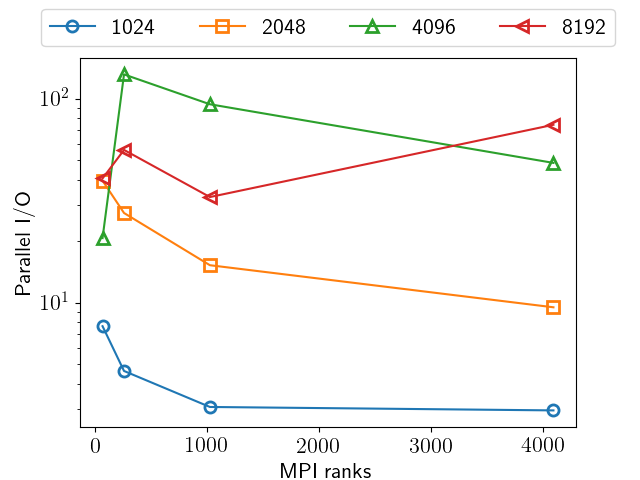
\includegraphics[scale=0.4]{Figures/cannon/io.png}
    \caption{ Parallel I/O time at different \# of MPI ranks for writing different matrix size (1024$\times$1024, 2048$\times$2048, 4096$\times$4096, 8192$\times$8192)}
    \label{cannon_io}
\end{figure}
% -------- Table: I/O ----------------
\newcolumntype{g}{>{\columncolor{Gray}}c}
\begin{table}[!ht]
\caption{Parallel I/O for different MPI ranks and matrix sizes} \label{cannon_tb_io} 
\centering
\begin{tabular}{c|g|g|g|g}
\hline
\rowcolor{white}
& \multicolumn{4}{c}{\# MPI ranks}\\
\hline
\rowcolor{white}
\# Matrix size &64 &256 &1024 &4096 \\
\hline
\rowcolor{white}
1024 & 7.657 & 4.619 & 3.076 & 2.960 \\

2048 & 39.567 & 27.477 & 15.240 & 9.477 \\
\rowcolor{white}
4096 & 20.702 & 131.345 & 93.756 & 48.368 \\

8192 & 40.583 & 56.003 & 32.896 & 74.382 \\
\hline
\end{tabular}
\end{table}

\newpage
\subsection{The Strip Algorithm}
% -------- Strip Algorithm ---------------- 
\subsubsection{Time Evaluation}
We evaluate the total running time, time for overheads, and real computational execution time of the strip algorithm. The results are shown below. Table \ref{te_algo1} displays the time of overheads (OH) and the real computational execution time (Exe) of our strip algorithm using the function \textbf{StripMatrix} and a combination of MPI and Pthreads. We also applied the $threads\_per\_rank = 1$, but due to the memory limit of the system, it is not able to be successfully executed. The excessive memory is due to the memory copy of MPI ranks. By comparing the overhead time and real computational execution time, we can see that, in general, the real time spent on computational work decreases as the number of processors increases and the higher threads per rank ratio leads to shorter time for computations if the total number of MPI ranks $\times$ threads per rank remains the same. For 4 threads per rank, the large differences in time for overheads among different number of compute nodes may be caused by the large number of MPI ranks when they wait for each other to generate the final result matrix. But actually, except for 4 threads per rank, time for overheads is very small compared to the real computational time and it does not change too much when the number of processors changes. 
%--------------------------------------------------------
% Table: Execution time for Algo1
%--------------------------------------------------------
\newcolumntype{g}{>{\columncolor{Gray}}c}
\begin{table*}[!ht]
\caption{Time for overheads (OH) and real compute execution time (Exe) (in seconds) using different number of compute nodes (Nds) for the strip algorithm } \label{te_algo1} 
\centering
\begin{tabular}{c|g|g|g|g|g|g|g|g|g|g}
\hline
\rowcolor{white}
& \multicolumn{10}{c}{\# Threads per Rank}\\
\hline
\rowcolor{white}
\multirow{2}{*}{Nds }&\multicolumn{2}{c|}{4} &\multicolumn{2}{c|}{8} &\multicolumn{2}{c|}{16} &\multicolumn{2}{c|}{32} &\multicolumn{2}{c}{64}\\\cline{2-11}
&OH &Exe &OH &Exe&OH &Exe&OH &Exe&OH &Exe\\\cline{2-11}
\hline
\rowcolor{white}
4&0.168421    &109.835415   &0.290572   &122.129506   &0.225283    &107.927725    &0.163505  &107.622015   &0.146021   &89.635461   \\
8& 6.337576   &59.591851   &0.700413   & 62.708707  &0.191444  &46.415216    &0.543975   &45.163827    &0.177769   &42.708561  \\
\rowcolor{white}
16&2.830000   &32.957763    &0.882918   &26.141934   & 0.885934  &22.474756    & 0.197669   &21.956846    &0.194354    &21.017222  \\
64& 6.213284    &11.681338    &0.392208  &6.927292   &0.248984  &5.772448     &0.205432   &5.543385   &0.204919    & 5.320643 \\
\rowcolor{white}
128&0.909988   &8.556207   &0.344109  & 3.349235   &0.207056   &2.977013    & 0.206682    & 2.817315    &0.207171   &2.704931   \\
\hline
\end{tabular}
\end{table*}

%--------------------------------------------------------
% Figure: Execution time for Algo1
%--------------------------------------------------------
The Figure \ref{exec_time} helps us visualize the total running time for 25 successful experiments. According to Figure \ref{exec_time}, in general, when the total number of MPI ranks and threads remains the same but the number of threads per MPI rank increases, the running time decreases since more computations are processed simultaneously. For each single graph line (i.e. with the same $threads\_per\_rank$ value), the running time also decreases when we use more compute nodes which leads to more total number of MPI ranks and threads. In general, when the number of compute nodes is doubled, the total time tends to be reduced to approximately half. The reason is that more work is done in parallel and thus the resource contention is reduced. This achieves the strong scaling since we compute a problem with the fixed size $N$ times faster than a single processor, where $N$ is the number of processors applied.
\begin{figure}[!h]
    \centering
    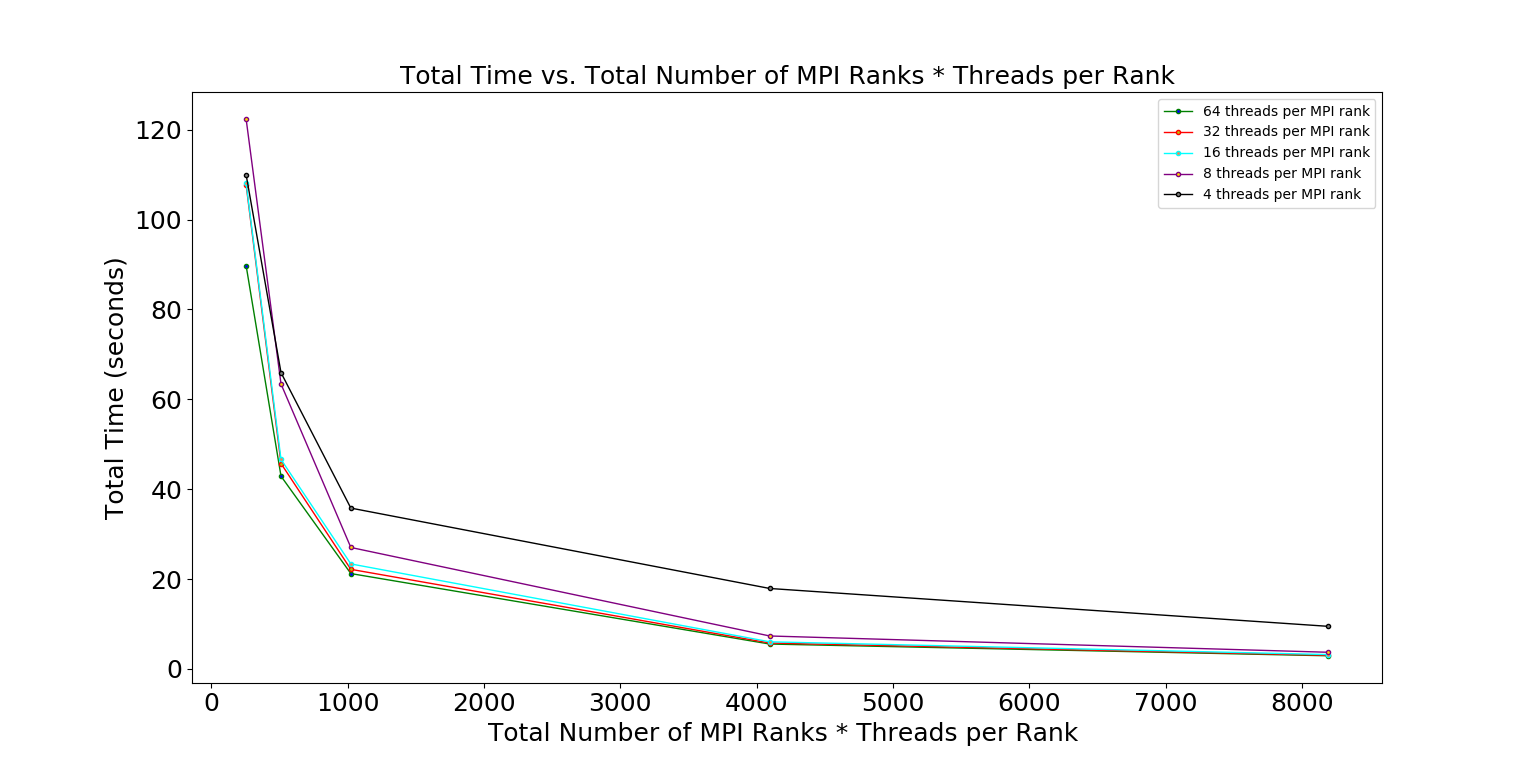
\includegraphics[scale=0.25]{Figures/exec_algo1.png}
    \caption{The total time (Y-axis) as a function of the total number of MPI ranks * threads per rank (X-axis) for 25 experiments. Each graph line is for a different value of $threads\_per\_rank$.}
    \label{exec_time}
\end{figure}

\subsubsection{Speedup Evaluation}
We chose the slowest experiment, which uses 4 compute nodes with $threads\_per\_rank = 8$ as the base case to be compared with other experiments. We compute the overall speedup using the formula (the total running time of 8 threads per rank using 4 compute nodes)/(the total running time of any one experiment). The Table \ref{se_algo1} shows the overall speedup of each experiment. 
%--------------------------------------------------------
% Table : Speedup for algo1
%--------------------------------------------------------
\newcolumntype{g}{>{\columncolor{Gray}}c}
\begin{table}[!ht]
\caption{Speedup values for the strip algorithm } \label{se_algo1} 
\centering
\begin{tabular}{c|g|g|g|g|g}
\hline
\rowcolor{white}
& \multicolumn{4}{c}{\# Threads per Rank}\\
\hline
\rowcolor{white}
\# Nodes &4 &8 &16 &32 &64 \\
\hline
\rowcolor{white}
4&1.113   &1.0   &1.132   &1.136      &1.364    \\
8&1.857    &1.931   &2.627  &2.678   &  2.855  \\
\rowcolor{white}
16&3.421   &4.530   &5.240  & 5.526 & 5.771   \\
64&6.841   &16.725   &20.331  &21.295  & 22.155 \\
\rowcolor{white}
128&12.932  & 33.146 &38.448  &40.483   &42.038    \\
\hline
\end{tabular}
\end{table}
%--------------------------------------------------------
% Figure : Speedup for algo1
%--------------------------------------------------------
In Figure \ref{speedup2}, the points are  grouped based on the same $threads\_per\_rank$  value. For the same number of MPI ranks and threads, 64 threads per MPI rank always works the best; for the same $threads\_per\_rank$ value, the maximum speedup is obtained when we use more processors.The reason is that more computational work is done in parallel by multiple processors and pthreads cause less overheads compared to MPI ranks. In this algorithm, the real computational execution time is dominant. As the threads per rank ratio increases, the speedup performs like a linear line. The reason is that less time is spent on MPI\_Barrier to wait all ranks to finish their work before proceeding to the next step. 
\begin{figure}[!h]
    \centering
    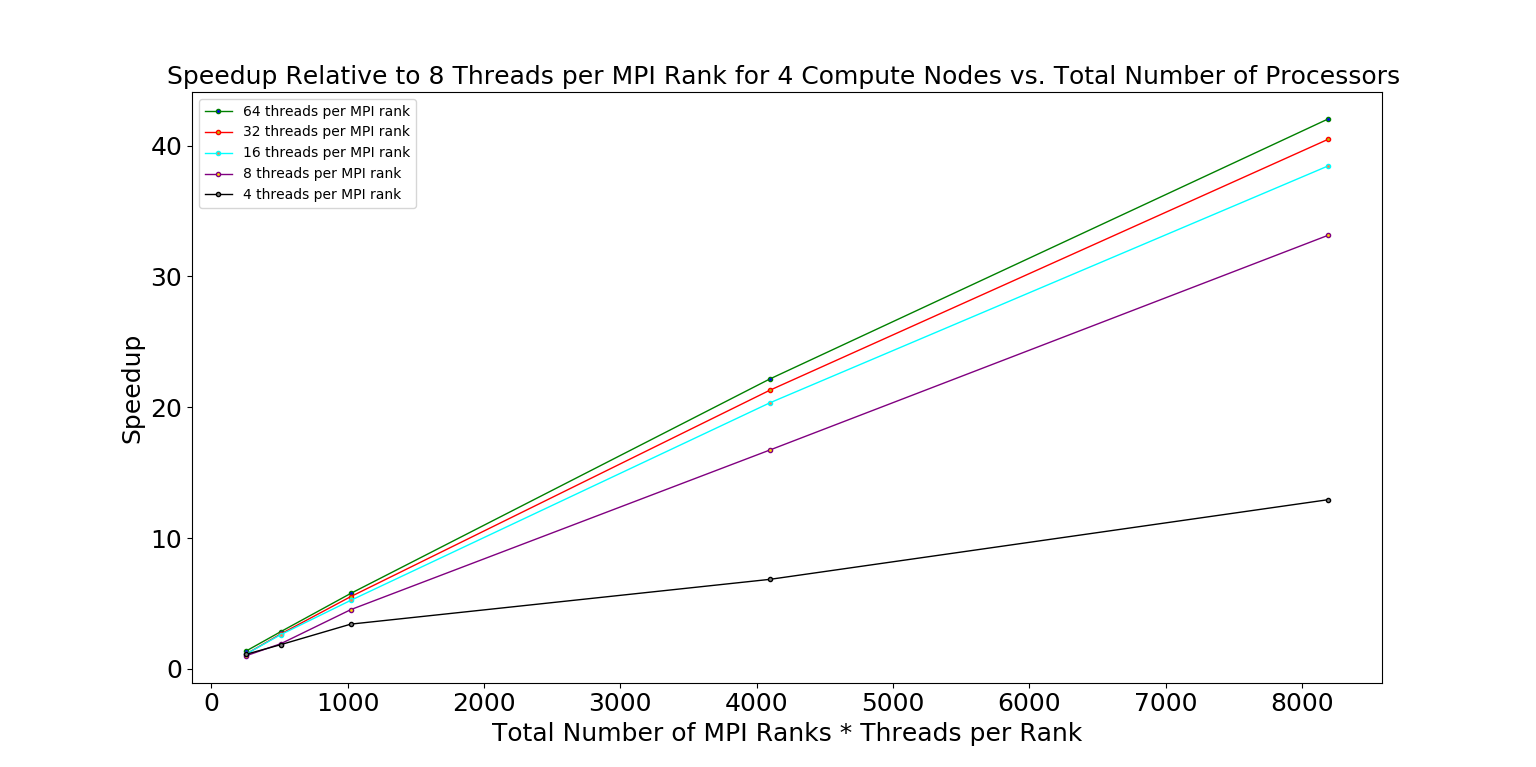
\includegraphics[scale=0.25]{Figures/speedup_algo1.png}
    \caption{The overall speedup of all experiments relative to the experiment using 8 threads per MPI rank for 4 compute nodes. Each graph line is for a different value of $threads\_per\_rank$.}
    \label{speedup2}
\end{figure}

\subsubsection{Parallel Efficiency Evaluation}
%--------------------------------------------------------
% Table : Parallel efficiency for algo1
%--------------------------------------------------------
Parallel efficiency is used to measure the utilization of resources and is calculated through dividing the speedup by the total number of processors. The Table \ref{pe_algo1} demonstrates the parallel efficiency of the experiments for the strip algorithm.
\newcolumntype{g}{>{\columncolor{Gray}}c}
\begin{table}[!ht]
\caption{Parallel efficiency values for the strip algorithm } \label{pe_algo1} 
\centering
\begin{tabular}{c|g|g|g|g|g}
\hline
\rowcolor{white}
& \multicolumn{4}{c}{\# Threads per Rank}\\
\hline
\rowcolor{white}
\# Nodes &4 &8 &16 &32 &64 \\
\hline
\rowcolor{white}
4& 0.00435  &0.00391   &0.00442   &0.00444  & 0.00533  \\
8& 0.00363   &0.00377   &0.00513  &0.00523   & 0.00558   \\
\rowcolor{white}
16&0.00334   &0.00442    &0.00512  &0.00540  & 0.00564   \\
64& 0.00167  &0.00408   &0.00496  &0.00520  & 0.00541 \\
\rowcolor{white}
128& 0.00158 &0.00405  &0.00469  &0.00494   &  0.00513  \\
\hline
\end{tabular}
\end{table}
%--------------------------------------------------------
% Figure : Parallel efficiency for algo1
%--------------------------------------------------------
According to the Figure \ref{efficiency}, the greatest parallel efficiency is achieved by 64 threads per MPI rank when we use the same number of processors; and among them, 16 compute nodes has the greatest parallel efficiency. The reason is that with more threads, more calculations can be done in parallel and using 16 compute nodes makes each processor perform optimally. Since the data communication for this strip algorithm is very little, the parallel efficiency is determined by the number of threads applied. Compared to MPI ranks, threads have less overhead and can directly communicate with others instead of through interprocess communication networks. As the number of threads per rank increases, the parallel efficiency is more stable and performs close to a horizontal line, which is ideal, as shown in the Figure  \ref{efficiency}. The slight decreasing trend is caused by the MPI overheads. The obvious decreasing trend for 4 threads per rank is due to the rapid increasing number of MPI ranks, which will generate a lot of overheads.
\begin{figure}[!h]
    \centering
    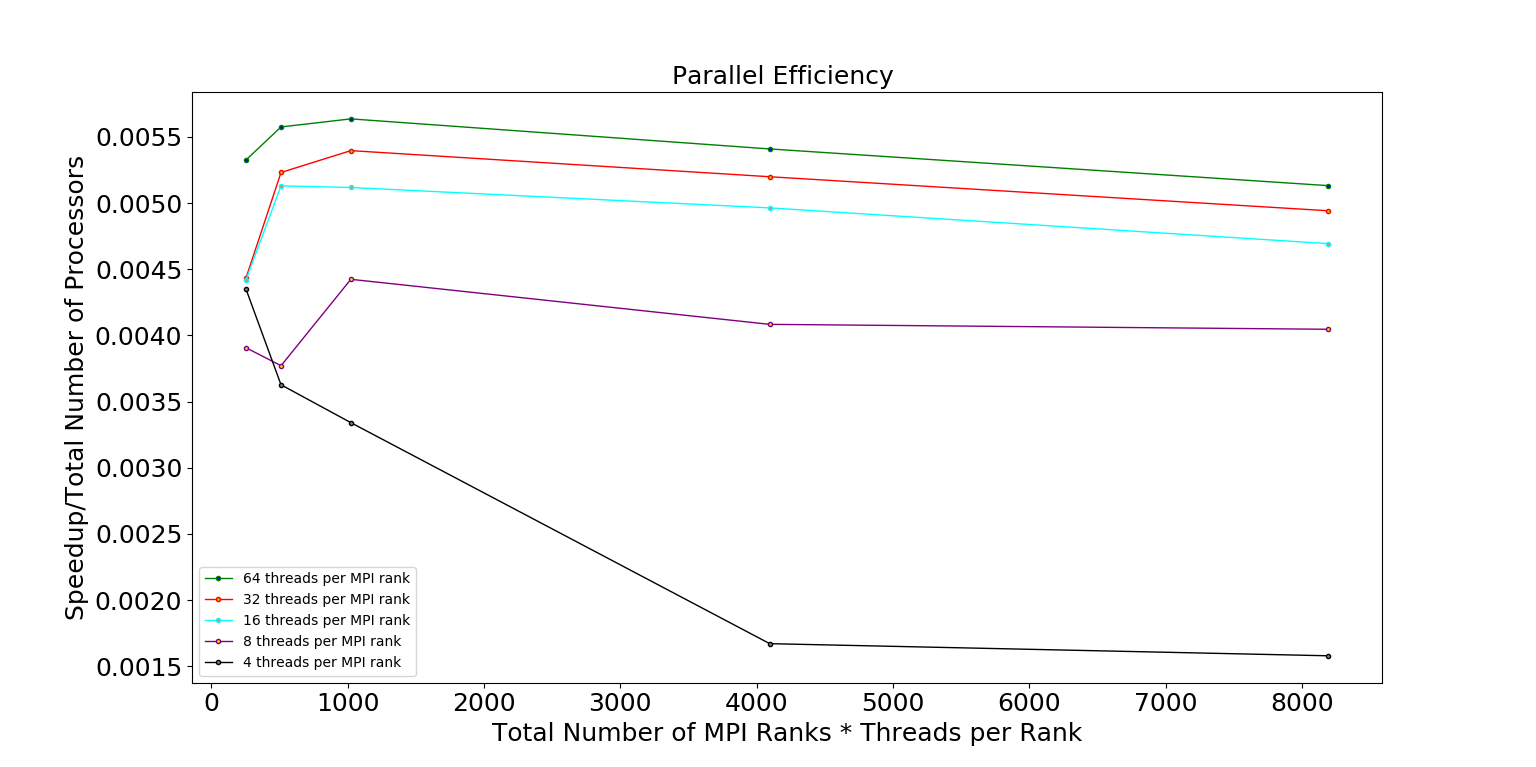
\includegraphics[scale=0.25]{Figures/efficiency_algo1.png}
    \caption{ Parallel efficiency for 25 experiments. Each graph line is for a different value of $threads\_per\_rank$.}
    \label{efficiency}
\end{figure}

\subsection{Comparison of two algorithms}
The execution time of Cannon's and Strip algorithms is listed in Table \ref{cannon_tb_comp_two_algs}, which indicates that our Strip algorithm runs much faster than conventional Cannon's algorithm. However, in spite of only containing a strip of matrix $A$ and generating a strip of local matrix $C$, it has to store the whole $B$ matrix for each MPI rank, which makes it memory inefficient. This even leads to the failure of running the case of one thread per rank (only MPI master thread runs without creating new thread) for matrix size of $8192\times8192$.
% -------- Table: Compare two algs ----------------
\newcolumntype{g}{>{\columncolor{Gray}}c}
\begin{table}[!ht]
\caption{Execution time of Cannon's algorithm and Strip algorithm with 4, 16, and 64 nodes} \label{cannon_tb_comp_two_algs} 
\centering
\begin{tabular}{c|g|g|g}
\hline
\rowcolor{white}
&\multicolumn{3}{c}{\# Nodes}\\
\hline
\rowcolor{white}
Algorithm & 4 & 16 & 64 \\
\hline
\rowcolor{white}
Cannon & 146.024 & 32.950 & 8.360 \\
Strip & 89.635 & 21.017 & 5.321 \\
\hline
\end{tabular}
\end{table}

\section{Conclusions}\label{conclusions}
We implemented two algorithms for matrix multiplication: conventional Cannon's algorithm and Strip algorithm proposed by ourselves. Both of these two algorithms have strong scalability and ideal parallel efficiencies when computing large size of matrices. Three types of overheads are identified for Cannon's algorithm and setting up Cartesian topology (not communication cost) is found to be the main overhead at high MPI ranks, which is counter intuitive. It was found that our Strip algorithm runs approximately 30\% faster than Cannon's algorithm by reducing the overheads including communication cost, initial matrices alignment, and creation of Cartesian topology.

\section{Future Work}\label{future_work}
As described above, Cannon's algorithm is memory efficient based on its checkboard data decomposition but it produces lots of overheads among processors and is hard to be implemented through the light weight Pthreads; in contrast, the strip algorithm has very few overheads but it consumes a large amount of memory. So, in the future, we could combine these two methods together to create a new algorithm that is both memory-efficient and with few overheads. To achieve it, we will replace the traditional sequential algorithm applied to local calculations in each processor used in Cannon's algorithm with the strip algorithm. In this way, the Cannon's algorithm can take advantage of Pthreads to maximize the parallel calculations while not increase the cost by overheads a lot. 

Furthermore, we will modify both algorithms to make them successfully work for non-square matrices since not all data matrices derived from real-life problems are square matrices. Besides directly modifying the two algorithms separately, we can combine them together to do the matrix multiplication for non-square matrices. We can decompose the non-square matrix into a square matrix and a rectangular matrix and then apply different methods on them to do the calculation. 

Moreover, currently, we assume that the data is equally divided to all processors; however, in the real-life problems, data are not able to be perfectly divided by the number of processors. So, it is reasonable to modify our algorithms to accept matrices with a size that is not divisible by the number of processors.

After implementing the above ideas, the new algorithm should become more practical and its range of application should be broader. And we can apply them to various real-life problems such as signal processing and weather pattern analysis \cite{b1} and compare with other existing efficient parallel matrix multiplication algorithms.

\section*{Acknowledgment}
We would like to thank our professor Dr. Carothers for his patient guidance and valuable suggestions during the semester. We also appreciate the help from our TAs Pras Date and Ridwan Al Iqbal.

\section*{Code Storage}
The absolute path for our code in Blue Gene/Q system is ``/gpfs/u/home/PCP8/PCP8fngj/scratch/matrix-multiplication". 

For Cannon's algorithm, please go to folder "cannon/" and run the commands below:
\begin{itemize}
    \item Compiling - \$ ./cannon\_alg\_compile.sh
    \item Executing - \$ ./cannon\_alg\_sbatch.sh num\_of\_nodes matrix\_rows time\_limit
    \item Plotting - \$ ./cannon\_alg\_plot.py
\end{itemize}

For Strip algorithm, please go to folder "strip/" and run the commands below:
\begin{itemize}
    \item Compiling - \$ ./strip\_alg\_compile.sh
    \item Executing - \$ ./strip\_alg\_sbatch.sh num\_of\_nodes threads\_per\_rank time\_limit
    \item Plotting - \$ ./strip\_alg\_plot.py
\end{itemize}

\begin{thebibliography}{00}
\bibitem{b1} V. Yegnanarayanan, ``An Application of Matrix Multiplication,'' Resonance, vol. 18, pp.368--377, April 2013.
\bibitem{b2}  Z.A.A. Alqadi, M. Aqel, and I. M. M. El Emary , ``Performance Analysis and Evaluation of Parallel Matrix Multiplication Algorithms,'' World Applied Sciences Journal, vol. 5, pp.211--214, January 2008.
\bibitem{b3} H.H. Abuazab , A.O. Dahmane, and H. Hamam1 , ``Sub Tasks Matrix Multiplication Algorithm (STMMA),'' World Applied Sciences Journal ,vol. 18, pp.1455--1462, 2012.

\bibitem{b4} Y. Li, and H. Li , ``Optimization of Parallel I/O for Cannon's Algorithm Based on Lustre,'' 11th International Symposium on Distributed Computing and Applications to Business, Engineering & Science ,2012. [Online].  Available: https://ieeexplore.ieee.org/abstract/document/6385233.

\bibitem{b5} M.Gilge, IBM System Blue Gene Solution Blue Gene/Q Application Development. International Business Machines Corporation, U.S., 2013.


\bibitem{b6} T. Lippert, N. Petkov, P. Palazzari, and K. Schilling, ``Hyper-systolic matrix multiplication,'' Parallel Computing,vol. 27, pp.737--759, May 2001.

\bibitem{b7} S. Lakhani, Y. Wang, A. Milenkovi, and V. Milutinovi , ``2D matrix
multiplication on a 3D systolic array ,'' Microelectronics Journal ,vol. 27, pp.11--22, 1996.


\bibitem{b8} B. M. Randjelovic, E. I. Milovanovic, and I. Z. Milovanovic , ``SYSTOLIC ALGORITHMS FOR MATRIX MULTIPLICATION ON SPACE OPTIMAL 1D SYSTOLIC ARRAYS,'' Ser. Math. Inform. ,vol. 29, pp.243--259, 2014.


\bibitem{b9}  G. Ballard, J. Demmel, O. Holtz, B. Lipshitz, and O. Schwartz , ``Communication-optimal parallel algorithm for strassen's matrix multiplication,'' ACM Symposium on Parallel Algorithms and Architectures, 2012. [Online].  Available: https://arxiv.org/abs/1202.3173.

\bibitem{b10} G.C. Fox, S.W. Otto, and A.J.G. Hey, ``Matrix algorithms on a hypercube I: Matrix multiplication,''Parallel Computing, vol. 4, pp. 17--31. 1987.


\bibitem{b11} E. Dekel, D. Nassimi, and S. Sahni, ``Parallel Matrix and Graph Algorithms,''SIAM Journal on Computing, vol.10, pp. 657--673, 1981. 

\bibitem{b12} J. Choi , J.J. Dongarra, and D.W. Walker,``PUMMA : Parallel Universal Matrix Multiplication Algorithms on Distributed Memory Concurrent Computers,'' Concurrency: Practice and Experience,1994. [Online].Available: http://citeseerx.ist.psu.edu/viewdoc/download?doi=10.1.1.55.6125&rep=\\rep1&type=pdf.

\bibitem{b13} J. Li, A. Skjellum, and R. D. Falgout, ``A poly-algorithm for parallel dense matrix multiplication on two-dimensional process grid topologies,'' Concurrency - Practice and Experience , vol.9, pp. 345--389, 1997. 

\bibitem{b14} S. Huss-Lederman  E. M. Jacobson, A. Tsao, and G. Zhang, ``Matrix multiplication on the Intel Touchstone Delta,'' Concurrency - Practice and Experience, vol.6, pp. 571--594, October 1994. 

\bibitem{b15} R. A. van de Geijn, and J. Watts, ``SUMMA: Scalable Universal Matrix Multiplication Algorithm,'' Concurrency - Practice and Experience, vol.9, pp.255–-274, April 1997. 

\bibitem{b16} A.Buluc, and J.R. Gilbert, ``PARALLEL SPARSE MATRIX-MATRIX MULTIPLICATION AND INDEXING: IMPLEMENTATION AND EXPERIMENT,'' SIAM J. SCI. COMPUT,vol. 34, pp. C170--C191, July 2012.

\bibitem{b17} J. Choi, ``A New Parallel Matrix Multiplication Algorithm on Distributed-Memory Concurrent Computers,''  Proceedings High Performance Computing on the Information Superhighway,1997. [Online].  Available: https://ieeexplore.ieee.org/document/592151.


\bibitem{b18} M. Krishnan , and J. Nieplocha, ``SRUMMA: a matrix multiplication algorithm suitable for clusters and scalable shared memory systems,''  18th International Parallel and Distributed Processing Symposium,2004.[Online].  Available:https://ieeexplore.ieee.org/document/1303000.


\bibitem{b19} R. Yuster, and U. Zwick, ``Fast Sparse Matrix Multiplication,''  Algorithms – ESA 2004 ,vol. 3221, pp.604--615, 2004.

\bibitem{b20} S. Ezouaoui , O. Hamdi-Larbi, and Z. Mahjoub , ``Dense-Sparse Matrix Multiplication : Algorithms and Performance Evaluation ,''  International Conference on Automation, Control, Engineering and Computer Science (ACECS'14), pp.87--94, 2014.

\bibitem{b21} M.J.Quinn, Parallel Programming in C with MPI and OpenMP. McGraw-Hill Education, Europe, 2008.

\bibitem{b22} F. L. Gall, ``Faster Algorithms for Rectangular Matrix Multiplication,''  IEEE 53rd Annual Symposium on Foundations of Computer Science,vol. 27, pp.737--759, October 2012. [Online].  Available:https://ieeexplore.ieee.org/document/6375330.




\end{thebibliography}


\end{document}
